\label{chap2}

This chapter describes the dynamic model derivation of the soft robotic manipulator. First, the soft robotic system used in this work is further detailed. Then the configuration space of the soft robot is described. Once this configuration space is determined, the forward kinematics at position and velocity level are derived. These forward kinematics allow to derive of the dynamic model of the soft robot. Additionally, a model is provided which will be used to capture the pump dynamics. Lastly, the state-space representation of the overall system dynamics is presented.


%%%%%%%%%%%%%%%%%%%%%%%%%%%%
%%%%%%%%%%%%%%%%%%%%%%%%%%%%f

\section{System description}

The soft robot studied in this work is composed of a visco-elastic polymer using selective laser sintering technology. This manufacturing method is well suited to print hollow compartments, that allow for inflation. The elastomer has a low Young's modulus and can sustain large strains. These characteristics allow inducing large deformations with relatively low pressures. The geometry of the soft robot is best described by two bellows placed in parallel. Over the vertical axis, the bellows are connected, creating the centre line of the actuator. The bellows are connected by flanges at the top and bottom. The bellows can be inflated individually via air inlets created in the flange at one end of the actuator. The other end is closed, allowing to pressurize the bellows. Since each bellow can be inflated independently, the entire actuator can increase its length and change orientation. Pressurizing both bellows equally will result in a near pure elongation of the soft robot. Creating a pressure difference will cause the soft robot's upper flange to rotate. The following assumption is made concerning the robot's task space:

\begin{theorem}
Strains in the soft robot imposed by pneumatic actuation change the soft robot's length and orientation. Strains causing out of plane motion are deemed negligibly small, and can not be actively controlled. The soft robot's task-space therefore restricts itself to the 2-dimensional plane.
\end{theorem}

This assumption allows describing the configuration of the soft robot in a two-dimensional Cartesian plane. Since the soft robot has no clear end-effector in the form of a gripper, a point on the body is assigned to be the end-effector. This point is situated at the geometric midst of the closed flange, see Figure \ref{fig2:setup}. The flange with the air inlets is fixed, here its geometric midst is defined as the origin. Altering the bellow pressure can therefore change the soft robot's end-effector position. Based on the above assumptions a kinematic model of the soft actuator is developed, based on the Cosserat beam model. 



\begin{figure}[H]
\begin{minipage}{.5\textwidth}
  \centering
  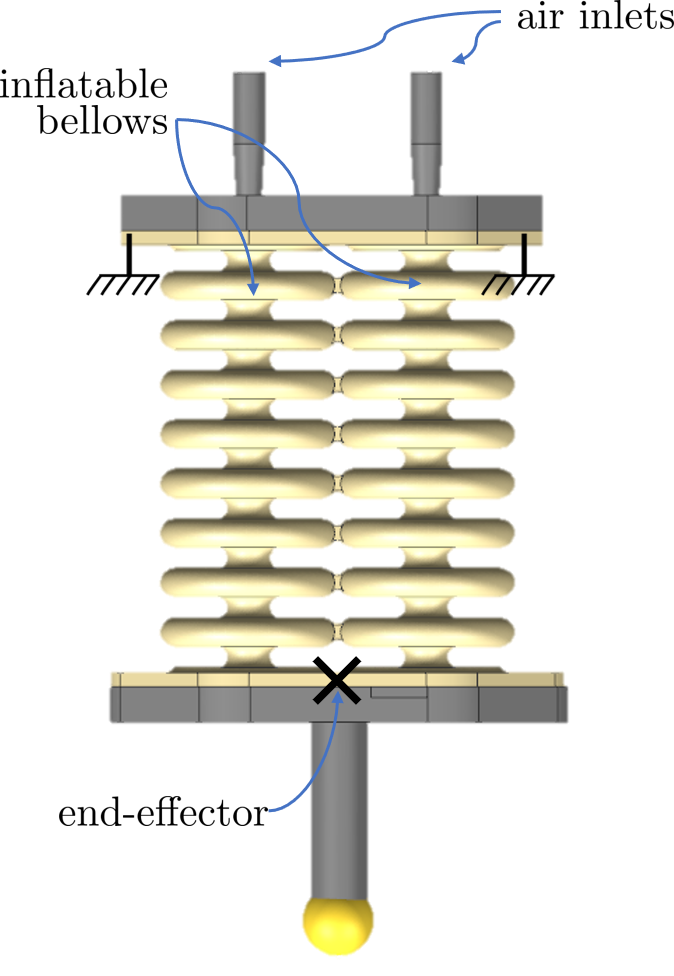
\includegraphics[width =0.8\linewidth]{Figures/Chapter2/setup.png}
  \caption{Schematic drawing of the actuator setup, denoting its fixation points and end-effector location.}
  \label{fig2:setup}
\end{minipage}
\begin{minipage}{.5\textwidth}
  \centering
    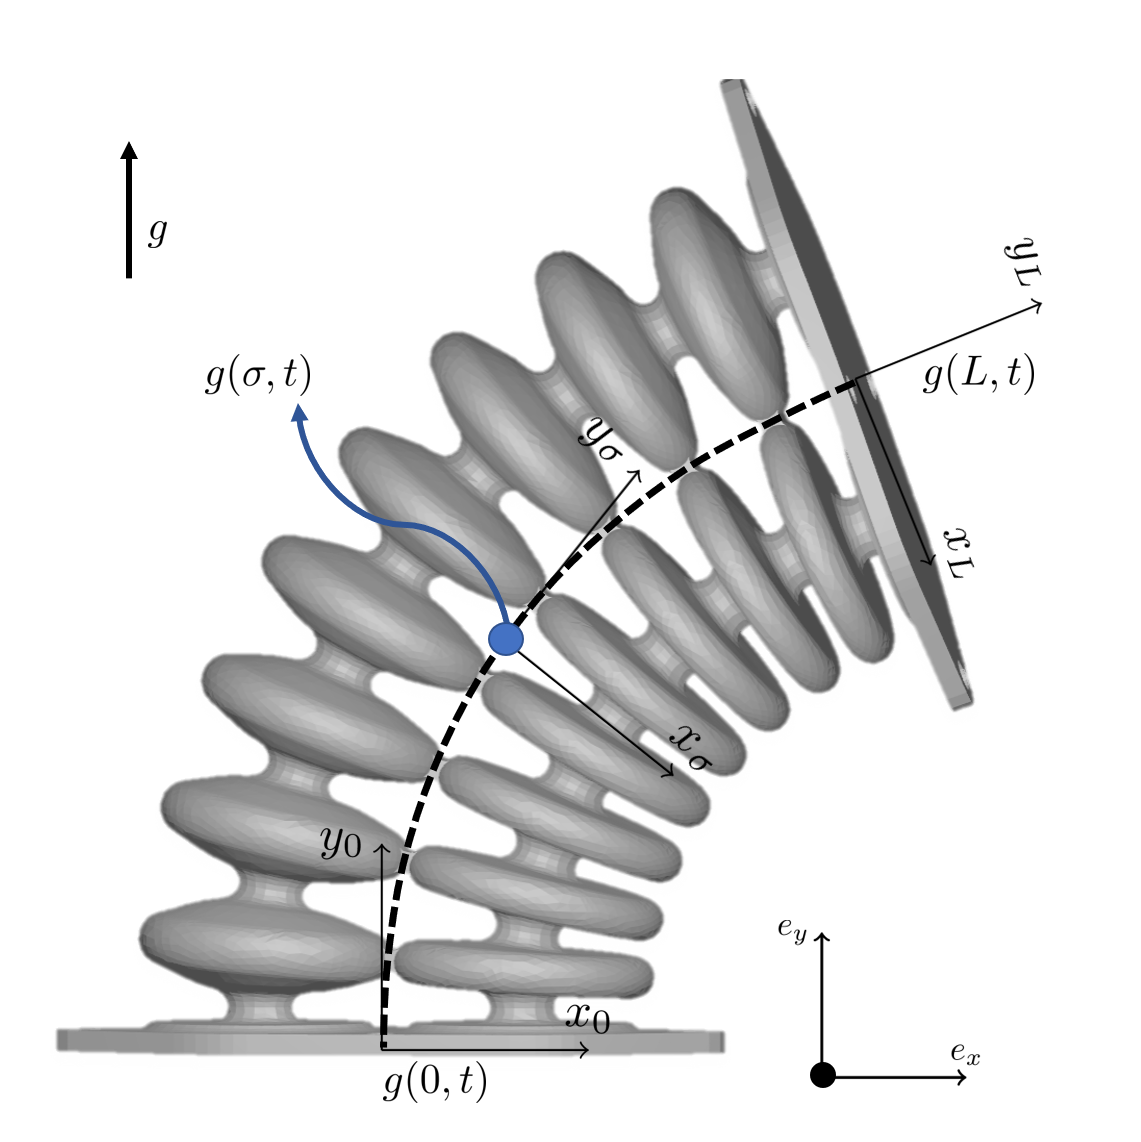
\includegraphics[width=\textwidth]{Figures/Chapter2/actuatorschematic.png}
    \vspace{15pt}
    \caption{Planar soft actuator with the backbone curve $g(\sigma,t)$.}
    \label{fig2:kinematicschematic}
\end{minipage}
\end{figure}





\section{Cosserat beam theory}

To describe the kinematics of the soft actuator, a Cosserat beam model is used \cite{Boyer2019}. This beam model can be thought of as a continuous one-dimensional curve representing the robot's backbone. This backbone is represented in Figure \ref{fig2:kinematicschematic} as the black dashed curve. This curve describes the configuration of the soft robot as a function of space and time. Therefore, this function is dependent on spatial coordinate $\sigma \in \mathbb{X}$ within bounded domain $\mathbb{X} \in [0,L_0] \subset \mathbb{R}$, where $L_0$ is the nominal length of the actuator. Furthermore, a temporal coordinate $t \in \mathbb{T}$ with $\mathbb{T} \in [0,T_{end}]$ is defined. Under the assumption that the soft robot's task space is a two-dimensional plane, the rotation of any point $\sigma$ at time instance $t$ is given by rotation matrix $R(\sigma,t) \in \mathbb{SO}(2)$. The matrices in $\mathbb{SO}(2)$ represent the special orthogonal group within Lie group theory. This matrix allows to express rotation of points on a two-dimensional surface, and is isomorphic to the circle group. Similarly, the position of that point is given by position vector $p(\sigma,t) \in \mathbb{R}^2$. Therefore, the Cosserat beam model creates a local frame at $\sigma$ which is tangential to this curve. This allows to describe position and rotation for any point $\sigma$ and time instance $t$ along the backbone of the soft manipulator by,


\begin{equation}
    g(\sigma,t) = \begin{bmatrix}  R(\sigma,t) & p(\sigma,t) \\ 0_3^\top & 1 \end{bmatrix} \in \mathbb{SE}(2),
    \label{eq2:g}
\end{equation}

where $\mathbb{SE}(2)$ represents the group of special euclidean matrices that represent rigid-body transformations on $\mathbb{R}^2$ \cite{Sola2018}. To derive forward kinematics, another assumption has to be made for this backbone curve $g(\sigma,t)$.

\begin{theorem}
Curve  $g(\sigma,t)$ is a continuous differential function $ \forall t \in 
\mathbb{T} $ and $\forall \sigma \in \mathbb{X}$
\end{theorem}

This assumption demands that derivatives of the backbone with respect to time and space are also continuous. These derivatives are essential in determining the strain and velocity field of the soft robot actuator. This strain field allows determining the time-invariant forward kinematics. Whilst the velocity field will be used in determining the system dynamics. First, we try to solve the forward kinematic problem by computing the strain field.



\section{Computation of the strain field}

The strain field allows us to study strains along the backbone curve. To find the strain we differentiate the backbone curve with respect to the spatial domain. Throughout this work derivatives with respect to the spatial domain will be indicated with a `prime', likewise time derivatives will be indicated with a `dot'. The local strain can be found by differentiating (\ref{eq2:g}) with respect to space. This results in the following partial differential equation (PDE), 

\begin{equation}
   g' = \frac{\partial g}{\partial \sigma} = g \hat{\xi} \hspace{10pt} \implies \hspace{10pt}  \hat{\xi}(\sigma,t) := g^{-1}g' = \begin{bmatrix} K_\times & E \\ 0_2^\top & 0 \end{bmatrix} \in  \mathfrak{se}(2)
    \label{eq2:dgdsigma}
\end{equation}

where $\hat{\xi}$ is the space-twist field. Here, $K_\times \in \mathfrak{so}(2)$ is a skew-symmetric matrix expressing single curvature strain. Since we consider a planar case, there is a rotation around a single axis. Therefore the skew-symmetric matrix is isomorphic to a scalar expressing the curvature, which we denote by $K_\times \longmapsto \kappa$. Furthermore, $E = [\epsilon_x,\epsilon_y]^\top \in \mathbb{R}^2$ containing stretch-shear strain. These skew-symmetric curvature strain and stretch-shear strain combined are within the Lie group $\mathfrak{se}(2)$ \cite{Sola2018}. Physically, $\kappa$ expresses the curvature of the actuator in the plane with unit $\kappa = 1/m$. The entries in vector $E$ represent shear in the horizontal direction and stretch in the vertical direction, respectively. It shall be clear that for the studied soft robot, shear or any other strain in the horizontal direction can not be actively controlled. Isomorphism of the Lie group $\mathfrak{se}(2)$ allows $\hat{\xi}(\sigma,t) \longmapsto \xi(\sigma,t)$. This allows to equivalently express these curvature strain and stretch-shear strain in a column vector as $\xi(\sigma,t) \in \mathbb{R}^3$ as $[\kappa \hspace{3pt} E^\top ]^\top$.

The PDE of \ref{eq2:dgdsigma} describes the forward kinematics, which is essential for computing the robot's configuration. It is useful to transform this PDE to an ordinary differential equation (ODE), as this allows for faster computation and controller design. This transformation reduces the system's original infinite dimensionality to a predefined dimension. To be able to transform the system, we make the following assumption: 

\begin{theorem}

$\forall t \in \mathbb{T}$ and $\forall \sigma \in \mathbb{X}$, strain $\xi(\sigma,t)$ can be written as an infinite expansion of the form \cite{Caasenbrood2021},

\begin{equation}
\xi_i(\sigma,t) = \sum_{k=1}^\infty \varphi_k(\sigma)q_{i,k}(t) + \xi_{i,0}(\sigma), \hspace{20pt} \forall \sigma \in \mathbb{X}, t \in \mathbb{T},
\label{eq2:strainexact}
\end{equation}

in which $\xi_{i}$ is the $i^{\text{th}}$ entry in the curvature-strain vector. Furthermore, $k \in \mathbb{N}^+$ is the index of the summation. The initial strains of the undeformed soft robot is given by $\xi_{i,0}$ and $\varphi_k(\sigma)$ is a set of basis shape functions evaluated at spatial instance $\sigma$ and $q_{i,k}(t)$ a column vector with modal coefficients. 
\end{theorem}

To be precise on this notation, each strain in column vector $\xi(\sigma,t)$ is described by an infinite summation. A single strain is denoted by $\xi_i(\sigma,t)$, with $i$ being the index of that strain. Column vector $q(t)$ contains modal coordinates for all strains in $\xi(\sigma,t)$ for each index $k$. Hence $\text{dim}(q(t)) = \text{dim}(\xi(\sigma,t)) \times \text{max}(k) = 3 \times \text{max}(k)$ . Column vector $\xi_{i,0}$ expresses the initial strain present in the undeformed system. Hence, $\text{dim}(\xi_0(\sigma)) = \text{dim}(\xi(\sigma,t))$.

This assumption allows transforming the PDE of (\ref{eq2:dgdsigma}) to an ODE by exploiting the Galerkin reduction method \cite{Galerkin}. Here, the infinite-dimensional system is projected onto a subspace of finite dimension that contains basis elements of the expected solution. Each of the three curvature/strains is approximated by a finite amount of shape functions each having a certain contribution to the complete solution. By reducing the dimensionality of the system, higher-order dynamics are not captured in the model and thus robustness should be taken into account. To transform the PDE in (\ref{eq2:dgdsigma}), the components of the strain field $\xi(\sigma,t)$ are approximated using a finite amount of shape functions as,

\begin{equation}
    [\xi_i(\sigma,t)]_N = \sum_{k=1}^N \varphi_k(\sigma)q_{i,k}(t) + \xi_{i,0}(\sigma), \hspace{20pt} \forall \sigma \in \mathbb{X}, t \in \mathbb{T},
    \label{eq2:strainapprox}
\end{equation}

where $N \in \mathbb{N}^+$ is the amount of truncations used to approximate strain $\xi_i(\sigma,t)$. Vector $q(t) \in \mathbb{R}^{3 \times N}$ only contains time-dependent modal coordinates. These modal coordinates can be viewed as coefficients expressing the contribution of individual mode shapes to the entire strain approximation. The modal coordinates used here are analogous to for example joint angles as used in traditional robotics. Furthermore, it should be clear that the initial internal deformation $\xi_{(i,0)}$ is time-invariant. For the studied soft robot the initial deformation is given as $\xi_0 = [0 \hspace{3pt} 0 \hspace{3pt} 1]^\top$. This means that the undeformed actuator is either in an upright or down configuration, e.g. no curvature $\kappa = 0$. Furthermore, the strain in horizontal direction $\epsilon_x = 0$. The stretch in vertical direction $\epsilon_y = 1$, which corresponds to the soft robots undeformed length $L_0$. The square brackets around $[\xi(\sigma,t)]_N$ indicate it is an approximation. 

There exist multiple variants of shape function polynomials that can be used in approximating strain. Here consider the Legendre polynomials as given by,

\begin{equation}
    \varphi_{k} = \frac{1}{2^{k-1} k-1!} \frac{d^{k-1}}{d\sigma^{k-1}}(\sigma^2-1)^{k-1},
    \label{eq2:shapefunction}
\end{equation}

here it can be seen that first Legendre polynomial is of zero-other, and results in 1 for $k=1$. Each degree of shape-function gives the model a certain amount of flexibility. Therefore increasing the order of shape functions allows the model to describe more complex robot configurations. To avoid coupling between the states, these shape functions must be orthogonal to each other. This means that $\int_\mathbb{X} \varphi_i \varphi_j d \sigma = 0$ for any $i \neq j$ and non-zero otherwise. The strain approximation of \ref{eq2:strainapprox} can be written as a $N$-th order expansion as,



\begin{equation}
\begin{aligned}
    \begin{bmatrix}\xi(\sigma,t)\end{bmatrix}_N = & \hspace{5pt}  (B_a \otimes [ \varphi_1(\sigma) \dots \varphi_N(\sigma) ])q(t)\\ = &  \underbrace{ \begin{bmatrix}
    \varphi_1(\sigma) & \dots  & \varphi_N(\sigma) & \dots     & 0      & \dots  &  0 \\
    \vdots    & \ddots & \vdots    & \ddots    & \vdots & \ddots & \vdots \\
    0         & \dots  & 0         & \dots     & \varphi_1(\sigma) & \dots & \varphi_N (\sigma)
    \end{bmatrix}}_{\Phi(\sigma)} \begin{bmatrix} q_{1,1}(t) \\ \vdots \\ q_{3,N}(t) \end{bmatrix} +  \begin{bmatrix} \xi_{1,0} \\ \vdots \\ \xi_{3,0}   \end{bmatrix}
    \end{aligned},
\label{eq2:xishape}
\end{equation}

where $\Phi(\sigma) \in \mathbb{R}^{3 \times mN}$ is the Kronecker-product between matrix $B_a \subseteq \text{span} \hspace{2pt} \mathbb{I}_3$ and vector $\varphi(\sigma) \in \mathbb{R}^N$. Here $m$ is defined as the number of active strains in the system. The definition of active strains in this context are strains that can be actively controlled. For our soft robot, this is the curvature $\kappa$ and the vertical elongation $\epsilon_y$. Hence, $m=2$ for our system. Based on these active strains, selection matrix of unconstrained strains can be defined as,

\begin{equation}
    B_a = \begin{bmatrix}
    1 & 0 \\
    0 & 0  \\
    0 & 1  \\
    \end{bmatrix}.
    \label{eq2:Ba}
\end{equation}

The entries of selection matrix $B_a$ tell us that only the first and third strain are free. This also implies that only these two strains are approximated. At this point, we have presented the forward kinematic problem and showed the Galerkin reduction method to approximate strains. This approximation allows formulating the system in finite-dimension. At this point we make another assumption regarding the maximum truncation in our strain approximation.

\begin{theorem}
The strains induced by actuating the soft robot under normal operation conditions can be captured by a truncation of $N = 1$. 
\end{theorem}

Based on this assumption, and the shape function polynomials of (\ref{eq2:shapefunction}) a first order approximation, e.g. $k=1$, will result in $\varphi_1 = 1$. Substitution of the provided expressions for $B_a$ (\ref{eq2:Ba}) and $\xi_0$ into (\ref{eq2:strainapprox}), the strains of the soft actuator can be described by,


\begin{equation}
    \begin{bmatrix}\xi(t)\end{bmatrix}_1 =\underbrace{B_a \otimes [\varphi_1]}_{\Phi(\sigma)} q(t) + \xi_0  =  \underbrace{\begin{bmatrix}
    1 & 0  \\
    0 & 0  \\
    0 & 1
    \end{bmatrix}}_{\Phi} \begin{bmatrix} q_{1,1}(t) \\  q_{2,1}(t) \end{bmatrix} +  \begin{bmatrix} 0 \\ 0 \\ 1   \end{bmatrix},
\label{eq2:xiapprox}
\end{equation}

where it can be seen that with a first-order strain approximation, the approximated strain becomes space-invariant. With this first-order approximation it holds that $B_a \otimes [\varphi_1] = \Phi(\sigma) \implies B_a = \Phi$, this will be used throughout this thesis. Furthermore, it can be seen that the second component of strain $[\xi(\sigma,t)]$, corresponding to elongation in x-direction it holds $\epsilon_x = 0 \hspace{3pt} \forall \hspace{3pt} \sigma $ and $ \forall \hspace{3pt} t$. This allows us to define the modal coordinates as,


\begin{equation}
q(t) = \begin{bmatrix} q_{1,1}(t) \\ q_{2,1}(t) \end{bmatrix} = \begin{bmatrix} \kappa(t) \\ \epsilon_y(t) \end{bmatrix} = \begin{bmatrix} \kappa(t) \\ \epsilon(t) \end{bmatrix},
\end{equation}

Since there is zero strain in the x-direction, we will agree upon a new signification for the strains. Throughout this work, we will use "elongation" or $\epsilon$ to address strain $\epsilon_y$. Likewise, ``curvature'', ``rotation'' or  $\kappa$ are used interchangeably to refer to curvature $\kappa$. Approximating strains and curvatures with a single shape function will reduce this Cosserat model to the piece-wise constant curvature (PCC) model as discussed in Chapter \ref{chapter1}. As can be seen from (\ref{eq2:shapefunction}), all shape functions yield 1 for $k=1$. In this case, the modal coordinates $q(t)$ will be equal to $\kappa$ and $\epsilon$, respectively. From this point onward, only a single shape function is used to approximate the strains and curvatures of the actuator. 

In the next section, the forward kinematic problem is solved with the described strain approximation.




\section{Forward kinematics}

The forward kinematic problem of \ref{eq2:dgdsigma} for the planar soft robot is programmed in \MATLAB \cite{MATLAB2020}. A standard ODE solver such as $\verb+ode45.m+$ can be used to solve the forward kinematic problem. The chosen initial condition is $g(0,t) = I_3 \hspace{2pt} \forall t$, which corresponds to zero rotation and zero strain at $\sigma = 0$. Furthermore, we choose our modal coordinates constant as $q = q(t) \hspace{2pt} \forall t$. This formulation allows us to integrate over the spatial domain $[0,L_0]$, as we assume time invariant behaviour. At each discrete increment the strain field $[\xi(t)]_1$ is approximated by (\ref{eq2:xiapprox}). 

Figure (\ref{fig1:forward_kinematic}) shows the result of the forward kinematic model. The initial position is obtained for zero curvature and elongation. Here it can be seen that the initial length of the actuator $L_0$ is equal to 64.5 mm. To obtain the deformed modal coordinate $q(t)$ was chosen equal to $[-17,0.1]^\top$. Physically this implies a clockwise rotation, creating an arc with a curvature of $17 \frac{1}{m}$, and elongation in the vertical direction of 10\%, which coincides with a measured arc-length of 70.9 mm.


\begin{figure}[H]
    \centering
    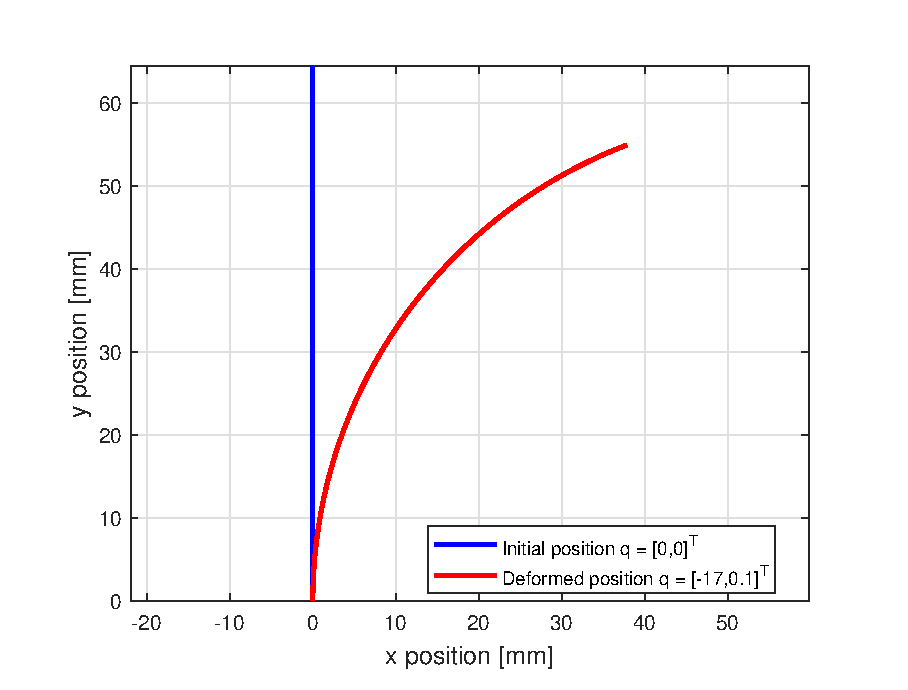
\includegraphics[width = 0.7\textwidth]{Figures/Chapter2/fkin1701.eps}
    \caption{Initial position and deformed position for a first order shape function approximation of the kinematic model.}
    \label{fig1:forward_kinematic}
\end{figure}

Besides a forward kinematic model, a numerical inverse kinematic solver was programmed. This allows defining a position in planar Cartesian coordinates, and obtain modal coordinates. The algorithm will minimize the distance between the desired end-effector position and reachable end-effector position given the amount of truncations $N$. It shows the model's flexibility when using multiple shape functions. The algorithm is further detailed in Appendix \ref{app:chap2}. 

For now, we have neglected the time dependency of modal coordinate vector $q(t)$. To determine the dynamics of the system it is crucial to consider the time variance of the system as well. To do so, we first consider the velocity kinematics of the system in the next section.


\section{Velocity kinematics}

The velocity kinematics allows us to study velocities along the backbone curve. Similar to the spatial derivative, backbone curve $g(\sigma,t)$ can be differentiated with respect to time. This differentiation results in, 

\begin{equation}
  \Dot{g} = \frac{\partial g}{\partial t} = g \hat{\eta} \hspace{10pt} \implies \hspace{10pt}  \hat{\eta} := g^{-1}\dot{g} = \begin{bmatrix} \Omega_\times & V \\ 0_2^\top & 0 \end{bmatrix} \in  \mathfrak{se}(2)
    \label{eq2:dgdt}
\end{equation}

which describes the time-twist field in a local frame at $\sigma$. Since we consider a planar case, there is a single angular velocity. Therefore the skew-symmetric matrix $\Omega_\times \in \mathfrak{so}(2)$ is isomorphic to a scalar expressing the angular velocity, which we denote by $\Omega_\times \longmapsto \omega$. Vector $V = [v_x,v_y]^\top \in \mathbb{R}^2$ contains linear velocities. Therefore, $\hat{\eta} \in \mathfrak{se}(2)$ effectively contains angular and linear velocities among the backbone curve. Due to the isomorphism of $\mathfrak{se}(2) \longmapsto \mathbb{R}^3$. All velocities can equivalently be stored in column vector $\eta(\sigma,t) = [\omega \hspace{5pt} V^\top]^\top \in \mathbb{R}^3$ \cite{Sola2018}.


Using the equality of mixed partial derivatives, at each instant of space and time $\frac{\partial}{\partial t}g' = \frac{\partial}{\partial \sigma}\dot{g}$ holds \cite{Caasenbrood2020}. By using general rules of substitution and actions in Lie space it can be proven that the spatial derivative of the velocity field can be written as,

\begin{equation}
    \eta'= (\text{Ad}_{g^{-1}})'\text{Ad}_g \eta + \Dot{\xi} \hspace{10pt} \text{with} \hspace{10pt} \text{Ad}_g = \begin{bmatrix} 0_2^\top & 1 \\ p_\times & R  \end{bmatrix} \in \mathbb{R}^{3\times 3}
    \label{eq2:etadif}
\end{equation}


where $\text{Ad}_g \in \mathbb{R}^{3 \times 3}$ \cite{2DLie} is the adjoint mapping of $g$ \cite{Sola2018}. Here, $p_\times$ is defined as $[p_2 \hspace{4pt} -p_1]^\top$ \cite{2DLie}, which can be derived from the adjoint action defined for the Lie group $\mathbb{SE}(3)$. The complete derivation of (\ref{eq2:etadif}) is presented in Appendix \ref{app:chap2}. 

An analytic solution to (\ref{eq2:etadif}) can be found by integrating the equation over spatial domain $[0,\sigma]$. It is given that the actuator is fixed at one end. Therefore the boundary conditions $\eta_0 = 0_{3 \times 1}$ and $g_0 = I_{3\times 3}$ can be imposed. This physically means that at $\sigma = 0$ there is no velocity, strain nor curvature. Integrating over domain $[0,\sigma]$ will give accordingly,

\begin{equation}
  \begin{bmatrix} \eta(\sigma,t)\end{bmatrix}_1 = \text{Ad}_{[g(\sigma,t)]_1^{-1}} \int_0^{\sigma} \text{Ad}_{[g(\sigma,t)]_1} \Phi d \sigma \dot{q}(t) = [J(\sigma,t)]_1\dot{q}(t),
    \label{eq2:J}
\end{equation}

here an expression for the geometric Jacobian $[J(\sigma,t)] \in \mathbb{R}^{3\times 2}$ is obtained \cite{Caasenbrood2020}. Note that we have approximated the strain with a first order truncation. This Jacobian maps modal coordinate velocity to linear and angular velocities along the backbone curve. Let us be clear on the dimension of this geometric Jacobian. Since we have two active degrees of freedom, that are strain $\epsilon$ in the y-direction and curvature strain $\kappa$, our modal coordinate vector $q(t)$ has length two. The geometric Jacobian maps the modal coordinate velocity $\dot{q}(t)$ to velocities in the Euclidean space. The velocity of a point with respect to a reference in 2-dimensional Euclidean space can be described by 3 components. From our fixed reference point at $g(0,t)$, these velocities are one rotational velocity, and two linear velocities in horizontal en vertical direction, respectively. As can be seen, this Jacobian matrix is non-linear with respect to position and time. Besides relating modal coordinate velocity to Cartesian velocity, the Jacobian can be used on position level as,

\begin{equation}
    r(\sigma,t) = [J(\sigma,t))]_1q(t),
\end{equation}

which implies that modal coordinates $q(t)$ can also be mapped to a position vector $r\in \mathbb{R}^3$ in Euclidean space. This position vector contains rotation, horizontal and vertical position as $[\theta \hspace{3pt} x \hspace{3pt} y]^\top$, respectively. Therefore this Jacobian is of valuable use for further system analysis. It can for instance be used in path-planning, as the Jacobian inverse can map Cartesian coordinates to modal coordinates. Furthermore, it can be used in controller design. However, in the next section, the Jacobian will be used for deriving the dynamics of the soft robot. 


\section{Dynamic model derivation}


To study the dynamic behaviour of the soft actuator a dynamic model is created. A relatively simple approximation is used to obtain insight into the basic dynamics of the actuator. The dynamic model will primarily be used for controller design. A relatively simple model is deemed to be sufficient to assess general controller performance. To this end, we propose a non-linear mass-spring-damper model. In the previous section, we obtained an expression for the Jacobian matrix. Here we observed its position and time variance, therefore it is assumed that the mass matrix of the system is also non-linear. Furthermore, it is known that the elastomer of which the soft actuator is composed deforms non-linearly. Therefore, the sought after form to describe our soft robot dynamics is,


\begin{equation}
    M(q(t))\Ddot{q}(t) + D\dot{q}(t) + K(q)q(t) = \nu(p,t),
    \label{eq2:simp_model}
\end{equation}


here $M(q) \in \mathbb{R}^{2\times 2}$ is the non-linear mass matrix. Furthermore, $D \in \mathbb{R}^{2\times2}$ is a linear damping matrix and lastly $K(q) \in \mathbb{R}^{2\times 2}$. It should be clear that the desired matrix dimensions correspond to length of modal coordinate vector $q(t)$. The input of the system is chosen $\nu(p,t) \in \mathbb{R}^2$, which is dependent on pressure and time. In this section we detail the derivation of each of these matrices. 

The dynamic model as presented in (\ref{eq2:simp_model}) can be obtained based on Lagrangian method given as $\mathcal{L} = \mathcal{T} -\mathcal{V}$. The Lagrangian $\mathcal{L}$ expresses the energy difference between kinetic energy $\mathcal{T}$ and potential energy $\mathcal{V}$. Exact expressions for the kinetic energy and potential energy of the system are given by, respectively,

\begin{equation}
    \mathcal{T} = \frac{1}{2}\int_0^{\sigma} \eta(\sigma,t)^\top \mathcal{M} \eta(\sigma,t) d \sigma \hspace{20pt} \text{and} \hspace{20pt}  \mathcal{V} = \frac{1}{2}\int_0^{\sigma} \xi(\sigma,t)^\top \mathcal{K} \xi(\sigma,t) d \sigma,
    \label{eq2:T}
\end{equation}


where $\mathcal{M} \in \mathbb{R}^{3\times3}$ and $\mathcal{K} \in \mathbb{R}^{3\times3}$ are a diagonal mass tensor and stiffness tensor, respectively. It should be noted that we have neglected gravitational effects contributing to the potential energy term. This is deemed valid as the system has a small mass. For the expression of the kinetic energy the velocity approximation of (\ref{eq2:J}) can be substituted. Additionally, the approximation of the strain field (\ref{eq2:xishape}) can be substituted in potential energy equation, this results in,

\begin{equation}
    \mathcal{T} = \frac{1}{2}\int_0^{\sigma} \Big([J(\sigma,t)]_1\dot{q}(t)\Big)^\top \mathcal{M} \Big([J(\sigma,t)]_1\dot{q}(t)\Big) d \sigma  \hspace{10pt} \text{and} \hspace{10pt}  \mathcal{V} = \frac{1}{2}\int_0^{\sigma} \big(\Phi q(t)\big)^\top \mathcal{K} \big(\Phi q(t)\big) d \sigma.
\end{equation}

These expression allows deriving the Lagrangian equations of motion as \cite{NWouw},

\begin{equation}
    \frac{\partial}{\partial t}\Big( \frac{\partial}{\partial\dot{q}}\mathcal{T}\Big)- \underbrace{\frac{\partial}{\partial q}\mathcal{T}}_0 + \frac{\partial}{\partial q}\mathcal{V} = \mathcal{Q}^{nc} \hspace{10pt} \text{with} \hspace{10pt} \mathcal{Q}^{nc} =  S\nu - \big(\Phi\dot{q}(t)\big)^\top \mathcal{D} \big( \Phi \dot{q}(t)\big)
    \label{eq2:lagrange}
\end{equation}

where $\mathcal{Q}^{nc} \in \mathbb{R^3}$ is a vector containing non-conservative forces acting on the system. One of these non-conservative forces are actuation forces. These actuation forces are captured in vector $\nu \in \mathbb{R}^2$, which is pre-multiplied with matrix $S \in \mathbb{R}^{3\times 2}$. This matrix $S$ represents the generalized direction of force and torque. In a moment we will prove this selection matrix is equal to matrix $B_a$. Another non-conservative force are the damping forces. Here damping tensor $\mathcal{D} \in \mathbb{R}^{3 \times 3}$. Also note that we have substituted the approximated strain velocity. Which without further prove is can be easily obtained from (\ref{eq2:xiapprox}). Furthermore we have assumed that the Coriolis effects $\frac{d}{dq}\mathcal{T}$ are zero. These Coriolis matrix contains terms $\dot{q}_i q_j$ with $i \neq j$. Since the entries of the mass matrix are small, and the dynamic system operates a low velocities this assumption is deemed valid. Further working out (\ref{eq2:lagrange}) gives,

\begin{equation}
    \int_0^\sigma \Big[ \underbrace{[J(\sigma,t)]^\top \mathcal{M} [J(\sigma,t)]}_{M(q)} \ddot{q}(t) +  \underbrace{\Phi^\top \mathcal{D} \Phi }_{D} \dot{q}(t)    +   \underbrace{\Phi^\top \mathcal{K} \Phi}_{K(q)} q(t)\Big] d\sigma = S\nu,
\end{equation}

here it becomes clear that $M(q)$, $D(q)$ and $K(q)$ are all in $\mathbb{R}^{2\times2}$. Recalling the generalized force and torque input vector $\Phi$, it can be concluded that $S = \Phi$ must hold. We are now further elucidating on finding the mass, damping and stiffness tensor, respectively.

In our modelling approach, the actuator kinematics have been described by a one-dimensional backbone curve. To derive the mass matrix, mass properties need to be assigned to this curve. Therefore the backbone curve is discretized, and we consider a cross-section of the actuator. In determining the mass of the system the following assumption is made.

\begin{theorem}
The inertial properties of the actuator can be determined by considering an infinitely thin slice in the transverse direction and regarding it as a solid cuboid.
\end{theorem}

Figure (\ref{fig:massapprox}) shows such a discretized cross section. Here the blue marked area is a solid cuboid with height $h$, width $w$, density $\rho$ and slice thickness $d\sigma$. 


\begin{figure}[H]
    \centering
    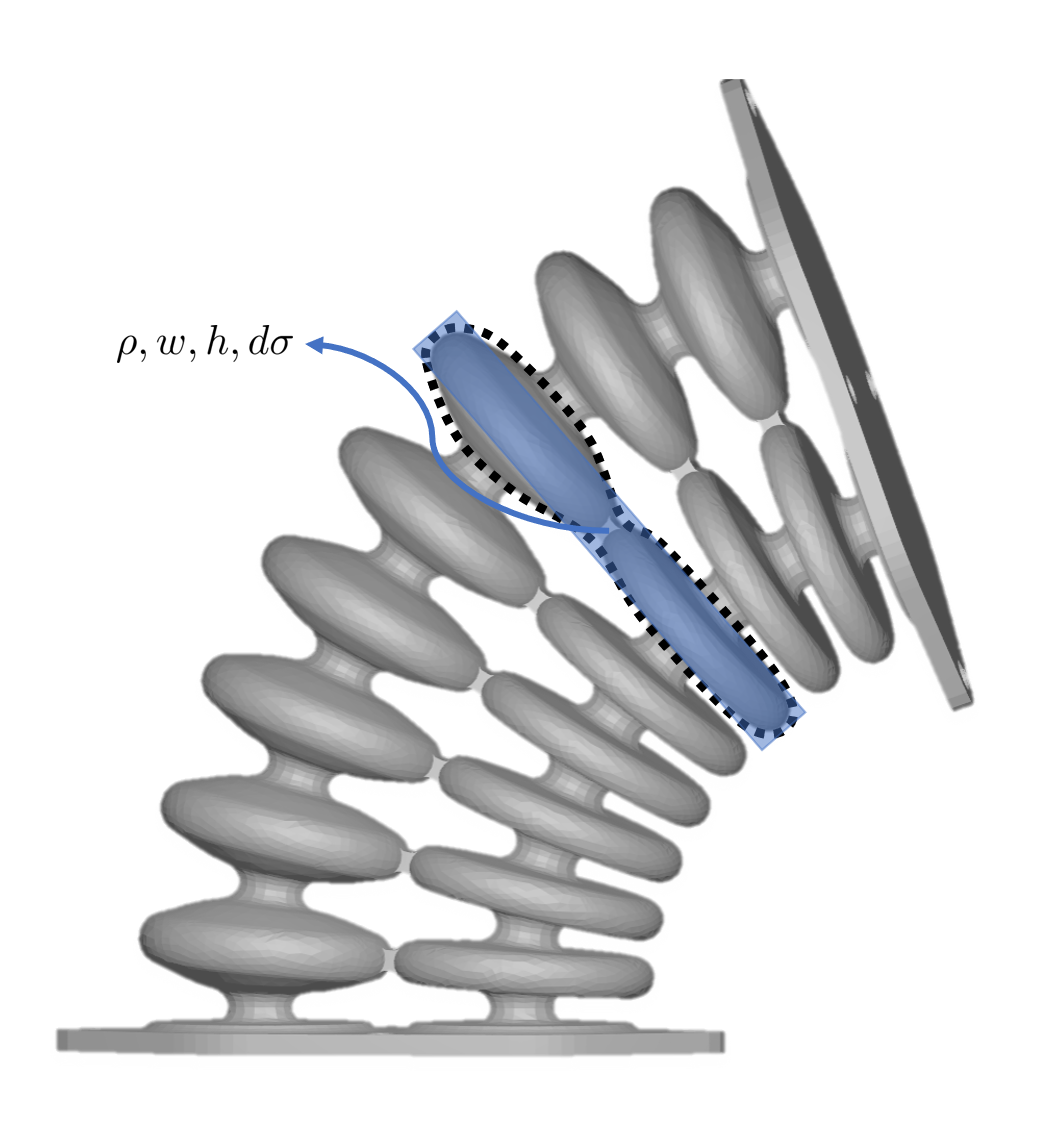
\includegraphics[width = 0.4\textwidth]{Figures/Chapter2/massapprox.png}
    \caption{Inertial properties can be determined by regarding an infinitely thin slice. The cross section is then viewed a solid cuboid.}
    \label{fig:massapprox}
\end{figure}


The mass tensor $\mathcal{M}$ then takes the following form,

\begin{equation}
    \mathcal{M} = \begin{bmatrix} \frac{1}{12}\rho (w^2 + d\sigma^2) & 0 & 0 \\
                                   0 & \rho & 0 \\
                                   0 & 0 & \rho \end{bmatrix}\hspace{5pt} \text{with} \hspace{5pt} \rho = \frac{m_{tot}}{L_0}
\end{equation} 




where $m_{tot}$ is the total mass of the actuator. The first entry expresses mass moments of inertia, related to the curvature of the actuator. The last three entries relate to linear velocities of the centre of mass of the cuboid. Based on equation (\ref{eq2:T}) the position variant mass matrix can be expressed as, 


\begin{equation}
    M(q) = \int_0^{\sigma} J(\sigma)^\top \mathcal{M}(\sigma)J(\sigma) d \sigma.
\end{equation}

Furthermore, damping and stiffness properties are assigned to the actuator. We assume that the polymer of which the actuator is made has linear damping characteristics. Therefore the damping matrix can be found as,

\begin{equation}
    D = \int_0^\sigma \Phi^\top \mathcal{D} \Phi d \sigma  = \text{diag}([D_\kappa, D_\epsilon])
\end{equation}.

Since it is hard to measure damping properties experimentally, the entries damping tensor will be chosen once doing simulations. Effectively, this means that we are trying to find damping parameters $D_\kappa$ and $D_\epsilon$. 

For a fact, we know that polymer has non-linear stiffness properties. Therefore stiffness matrix $K(q)$ is space-variant, and is therefore given by,

\begin{equation}
    K(q) = \int_0^\sigma \Phi^\top \mathcal{K}(q) \Phi  d\sigma, = \text{diag}([K_\kappa(q), K_\epsilon(q)]).
\end{equation}

Instead of defining the entries to the stiffness tensor $\mathcal{K}$, we have to determine the curvature stiffness $K_\kappa(q)$ and elongation stiffness $K_\epsilon(q)$. Determining these non-linear stiffnesses will be explained in Chapter \ref{chap3}. Furthermore, here the geometric properties and material properties will be given to determine the mass tensor. 




\section{Actuator dynamics}

At this point, we have derived a dynamic model for our soft actuator. However, actuation plays a dominant role in controlling our soft robot. Therefore it important to include pressure dynamics as well. To provide a complete dynamic model for analysing our controller, a pump model is derived. To this end, we assume that the pressure dynamics can be captured by a first-order linear dynamic model as,

\begin{equation}
    \dot{p}(t) = -\lambda_1 p(t) + \lambda_2 V(t),
\end{equation}

here $p(t)$ is the time-dependent pressure based on input voltage $V(t)$. Constant $\lambda_1 \in \mathbb{R}^+$ represents the system's resistance to a pressure increase and scales with actual system pressure. Parameter $\lambda_2 \in \mathbb{R}^+$ is a constant that incorporates the pressure increase relative to the volt input signal. Both of these parameters can be obtained by doing experimental analysis. This process is detailed in Chapter \ref{chap3}.



\section{Overall System dynamics}

The parameter identification allows to obtain the entries of mass matrix $M$ and stiffness matrix $K$. With the determined stiffness' matrix $K = \text{diag}([K_\kappa \hspace{3pt} K_\epsilon])$. The diagonal damping matrix is equal is represented by $D = \text{diag}([D_\kappa \hspace{3pt} D_\epsilon]) = \text{diag}([4e-5 \hspace{3pt} 0.3])$. Damping properties have not been determined experimentally, as the actuator cannot be actuated such that a measurable free excitation is induced in a single axis. Therefore the damping parameters are chosen iteratively. In Appendix \ref{app4}, a free oscillation of the dynamic model is presented. Here the effect of damping on the systems response is further elucidated. Furthermore an analysis on the accuracy of the model is provided.

The dynamic model of (\ref{eq4:SS}) allows for numeric solving by reformulating the model to a second order state-space formulation as,

\begin{equation}
     \begin{bmatrix} \dot{x}  \end{bmatrix}   = \underbrace{  \begin{bmatrix} O_2 & I_2 \\ -M(q)^{-1}K(q)  & -M(q)^{-1} D \end{bmatrix}   }_{A} \begin{bmatrix} x \end{bmatrix}  +      \underbrace{\begin{bmatrix} O_2 \\ M(q)^{-1}H   \end{bmatrix}   }_{B}    \begin{bmatrix} p_1\\ p_2  
     \end{bmatrix}, 
     \label{eq4:SS}
\end{equation}

with state vector $x = \begin{bmatrix} \kappa \hspace{3pt} \epsilon \hspace{3pt} \dot{\kappa}  \hspace{3pt} \dot{\epsilon}  \end{bmatrix}^{\top}$. Here matrix $A \in \mathbb{R}^{4\times 4}$ contains all elements with respect to the system dynamics. Matrix $B\in\mathbb{R}^{4 \times 2}$ is the control input vector. Mind the substitution of the mapping matrix, hence control input is pressure instead of force and moment. 

Above state-space does not allow to give an accurate system description as the pump dynamics are not included in this representation. Therefore an adapted state space formulation is presented as,

\begin{equation}
     \begin{bmatrix} \dot{x}  \end{bmatrix}   =   \underbrace{ \begin{bmatrix} O_2 & I_2 & O_2 \\ -M(q)^{-1}K(q)  & -M(q)^{-1} D & O_2 \\
     O_2 & O_2    & -\frac{1}{\tau_s(V)}I_2\ \end{bmatrix}   }_A   \begin{bmatrix} x \end{bmatrix}  + \underbrace{      \begin{bmatrix} O_2 & O_2 \\ M(q)^{-1}H & O_2 \\ O_2 & \frac{K(V)}{\tau_s(V)} I_2 \end{bmatrix} }_B      \begin{bmatrix} p_1 \\ p_2  \\ V_1 \\ V_2 \end{bmatrix},
     \label{eq:ssp}
\end{equation}







%\begin{figure}[H]
%        \centering
%        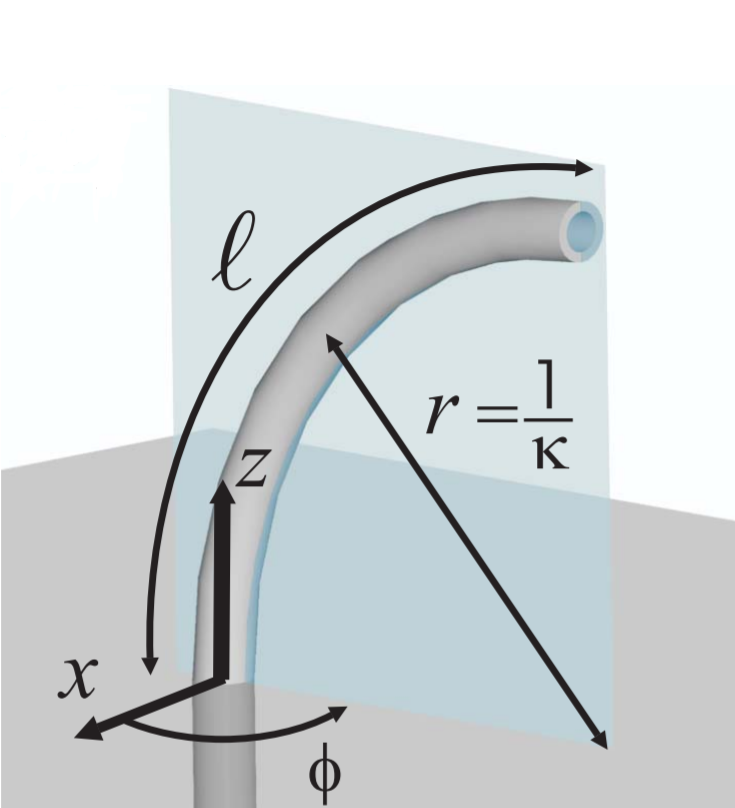
\includegraphics[width=0.85\linewidth]{Figures/Chapter2/ccapproach.png}
%         \caption{Schematic drawing of the constant curvature \cite{ccapproach}.}
%         \label{fig2:ccapproach}
%\end{figure}

